% !TeX program = xelatex
% 赤峰学院学报（自然科学版）规范格式论文
% 依据《赤峰学院学报（自然科学版）规范格式论文模板》排版
\documentclass[UTF8,a4paper,12pt]{ctexart}

% ==================== 基础宏包 ====================
\usepackage{geometry}
\geometry{top=2.4cm,bottom=2.4cm,left=2.5cm,right=2.5cm}

\usepackage{graphicx}
\usepackage{booktabs}
\usepackage{array}
\usepackage{amsmath,amssymb,bm}
\usepackage{siunitx}
\usepackage{caption}
\usepackage{subcaption}
\usepackage{enumitem}
\usepackage{setspace}
\usepackage{indentfirst}
\usepackage{titlesec}
\usepackage{natbib}
\usepackage[hidelinks]{hyperref}
\usepackage{tikz}
\usetikzlibrary{shapes.geometric,arrows.meta,positioning}

% ==================== 排版设置 ====================
\setlength{\parindent}{2em}
\setlength{\parskip}{0pt}
\linespread{1.25}

% 图表题：中文在前、英文在后
\captionsetup{
  font=small,
  labelsep=space,
  justification=centering,
  singlelinecheck=false
}

% 一级、二级、三级标题
\titleformat{\section}{\heiti\zihao{4}}{\thesection}{0.8em}{}
\titleformat{\subsection}{\heiti\zihao{-4}}{\thesubsection}{0.8em}{}
\titleformat{\subsubsection}{\heiti\zihao{-4}}{\thesubsubsection}{0.8em}{}

% 参考文献采用顺序编码制、方括号、上标形式
\setcitestyle{numbers,square,super,sort&compress}

% ==================== 自定义命令 ====================
\newcommand{\zhabstract}[1]{%
  \noindent\textbf{摘\quad 要：}#1\par
}
\newcommand{\zhkeywords}[1]{%
  \noindent\textbf{关键词：}#1\par
}
\newcommand{\clc}[1]{%
  \noindent\textbf{中图分类号：}#1\par
}

\newcommand{\enauthor}[1]{%
  \begin{center}
    #1
  \end{center}
}

\newcommand{\enabstract}[1]{%
  \noindent\textbf{Abstract: }#1\par
}
\newcommand{\enkeywords}[1]{%
  \noindent\textbf{Keywords: }#1\par
}

% 双语图题：\bicaption{中文图名}{English caption}
\newcommand{\bicaption}[2]{%
  \caption{#1\\[-0.2em]\small Fig.\thefigure\ #2}
}

% 双语表题：\bitablecaption{中文表名}{English table title}
\newcommand{\bitablecaption}[2]{%
  \caption{#1\\[-0.2em]\small Table \thetable\ #2}
}

\begin{document}

% ==================================================
% 题名区（不超过25字）
% ==================================================
\begin{center}
{\heiti\zihao{2}\textbf{光栅扭矩测量全链路建模与解调算法性能分析}\par}
\vspace{0.8em}

{\zihao{4} 张三$^{1}$，李四$^{2}$，王五$^{2}$\par}
\vspace{0.5em}

{\zihao{-5}
（1. 赤峰学院 物理与电子信息学院，内蒙古 赤峰 024000；2. 清华大学 精密仪器系，北京 100084）
\par}
\end{center}

\vspace{0.8em}

% ==================================================
% 中文摘要（不少于300字；结构：背景/问题→目的→方法→结果→定量数据→结论→创新点）
% ==================================================
\zhabstract{针对光栅扭矩测量中机械参数、光栅相位和四相接收信号相互耦合的问题，本文建立一套可追溯的离线数字孪生模型，分析非理想四相信号下不同解调方法的误差边界。模型依次描述扭矩—扭转角—切向位移—光学相位—四通道电压的映射，并在通道幅值、相位、偏置和高斯噪声扰动下，对专利基准的1/4、1/16、1/32计数细分、差分反正切和现有白化校正方法进行比较。基于MATLAB脚本的14个预定义工况离线计算表明：三十二细分方法的平均位移RMSE为$0.384\,\mathrm{\mu m}$，最大值为$0.728\,\mathrm{\mu m}$；差分反正切和现有校正方法的最大RMSE分别为$5.698\,\mathrm{\mu m}$和$7.748\,\mathrm{\mu m}$。在$-20~^\circ\mathrm{C}\sim80~^\circ\mathrm{C}$的参数敏感性仿真中，完整相位链的灵敏度相对变化为$-1.186\%\sim+1.833\%$，未补偿扭矩RMSE最大为$0.0847\,\mathrm{N\cdot m}$；采用同一温度模型的逆变换后，补偿误差降至双精度数值误差量级。上述结果仅代表\texttt{simulation/default}参数下的离线模型和算法对比；Stage 14的算法比较直接使用模拟通道，未经过ADC量化，也未完成实物标定或在线硬件验证。}

\vspace{0.4em}
\zhkeywords{光栅扭矩传感器；数字孪生；多物理场建模；四相信号细分；温漂补偿；鲁棒性评估}
\clc{TP212.14；TH741}

\vspace{1em}

% ==================================================
% 英文信息（与中文严格对应）
% ==================================================
\begin{center}
{\bfseries\large Full-Pipeline Modeling and Demodulation Performance Analysis for Optical Grating Torque Measurement\par}
\vspace{0.6em}
ZHANG San$^{1}$, LI Si$^{2}$, WANG Wu$^{2}$\par
\vspace{0.4em}
\small
(1. College of Physics and Electronic Information, Chifeng University, Chifeng 024000, China;\\
2. Department of Precision Instrument, Tsinghua University, Beijing 100084, China)
\end{center}

\enabstract{This study develops a traceable offline digital-twin model for optical grating torque measurement and evaluates demodulation under non-ideal four-phase signals. The forward chain maps torque to torsion angle, tangential displacement, optical phase, and four-channel voltage. Patent-reference 1/4, 1/16, and 1/32 counting subdivision, differential atan2, and an existing whitening-based correction are compared under the 14 cases implemented by the MATLAB benchmark script. The 1/32 method gives a mean displacement RMSE of $0.384\,\mathrm{\mu m}$ and a maximum of $0.728\,\mathrm{\mu m}$; the maximum RMSEs of differential atan2 and the existing correction are $5.698\,\mathrm{\mu m}$ and $7.748\,\mathrm{\mu m}$, respectively. A temperature-parameter sensitivity simulation from $-20~^\circ\mathrm{C}$ to $80~^\circ\mathrm{C}$ produces a full phase-chain sensitivity variation of $-1.186\%$ to $+1.833\%$ and an uncompensated torque RMSE up to $0.0847\,\mathrm{N\cdot m}$. Inverting the same temperature model reduces the simulated residual to floating-point round-off. These results are limited to offline \texttt{simulation/default} assumptions: the Stage 14 comparison uses analog simulated channels before ADC quantization, and no physical calibration or online hardware validation is claimed.}

\vspace{0.4em}
\enkeywords{optical grating torque sensor; digital twin; multi-physics modeling; four-phase signal subdivision; temperature drift compensation; robustness evaluation}

\vspace{1em}

% ==================================================
% 引言（不编号，不包含图、表、公式）
% ==================================================
\section*{引言}

扭矩作为旋转机械动力传输与状态监测的核心物理量，其高精度、高动态响应的在线实时测量在高端数控机床、新能源汽车动力总成、航空航天推进系统以及大型风力发电机组中发挥着决定性作用。相比于传统的电阻应变片式与压磁式扭矩传感器，基于莫尔条纹原理的光栅扭矩传感器具有非接触检测、抗电磁干扰能力强、测量分辨率高以及动态频响宽等显著优势，成为精密测控领域的研究热点之一\cite{ref1,ref2}。

在光栅传感测量系统中，读数头接收到的光电信号质量直接决定了最终的位移与角度解调精度\cite{ref3,ref4}。然而，在实际工业服役工况下，由于光源发光强度波动、光敏探测器响应不均、机械安装偏心及刻线制造缺陷，光电转换输出的正交莫尔条纹信号往往不可避免地掺杂直流偏置、幅值失配、正交相位畸变以及高次谐波等非理想误差\cite{ref5,ref6}。针对上述非线性误差，国内外学者先后提出了Heydemann椭圆参数拟合算法\cite{ref9}、改进粒子群优化校正法\cite{ref8}以及后验滤波补偿模型\cite{ref11}。但这些算法大多基于理想稳态或单一静态误差假设展开，对于强工业噪声干扰、反向动态突变以及零扭矩静态奇异等极限工况下的适应性缺乏系统性横向横评。

更为关键的是，光栅扭矩传感器是典型的力-光-机-电深度耦合精密系统。环境温度的显著剧变将同时改变扭轴材料的剪切弹性模量和光栅基底的微观刻线周期，使得系统宏观测量灵敏度发生非线性漂移。传统基于物理样机的静态离线标定方法试验周期漫长、开发成本高昂，且难以在多变服役现场实现实时在线解耦与动态补偿\cite{ref7,ref10}。近年来兴起的数字孪生技术通过构建物理实体在虚拟空间的高保真数字映射，为全生命周期性能评估、极端工况虚拟测试以及在线智能补偿提供了全新的技术途径。

鉴于此，本文针对一种基于同心圆环光栅的转动体扭矩测量系统，构建可追溯的离线数字孪生仿真链路。本文的主要工作包括：
（1）建立从扭轴力学变形、圆弧光栅微位移调制、光电探测到非理想信号注入与ADC量化的参数化模型；
（2）按 `stage14\_comparison.m` 的实际 `build\_cases` 构建14类离线工况，比较专利多相细分、差分反正切和现有白化校正算法；
（3）给出温度参数模型对扭转—相位灵敏度的影响，并验证同一模型逆变换的数值补偿效果；
（4）单独说明ADC和四通道串口帧模块的接口边界，不把协议帧生成等同于物理硬件通信。

% ==================================================
% 1 扭矩光栅传感器全链路数字孪生体系架构与物理模型
% ==================================================
\section{扭矩光栅传感器全链路数字孪生体系架构与物理模型}

\subsection{系统工作原理与多物理场架构}
本文研究的光栅扭矩测量系统主要由扭轴受扭弹性段、固定测量腔体、主光栅盘、指示光栅副、聚光准直光源、五路光电探测阵列以及温度传感模块组成。主光栅随扭轴变形端产生相对转角，与固定在测量腔体上的指示光栅形成重叠调制，进而产生随扭矩变化的周期性光强调制。

数字孪生仿真链路的总体架构如图\ref{fig:arch}所示。模型按“扭矩激励 $\to$ 机械微变形 $\to$ 光学相位调制 $\to$ 四通道模拟信号 $\to$ 误差注入 $\to$ ADC量化（独立接口）$\to$ 四通道串口帧（独立接口）”组织。图中后端接口用于定义数据边界；Stage 14算法统计直接使用误差注入后的模拟通道，并未经过ADC量化。

\begin{figure}[htbp]
  \centering
  \begin{tikzpicture}[node distance=1.0cm and 0.8cm, auto, >=Stealth,
    block/.style={rectangle, draw=black, thick, fill=white, text width=2.4cm, text centered, minimum height=1.1cm, font=\small},
    line/.style={draw=black, thick, -{Stealth[length=2.5mm]}}]

    \node [block] (input) {输入激励\\扭矩 $T$ / 温度 $T_{\mathrm{e}}$};
    \node [block, right=of input] (mech) {机械扭转层\\扭转角 $\theta$\\相对位移 $x_{\mathrm{rel}}$};
    \node [block, right=of mech] (opt) {光学调制层\\微位移透射\\光学相位 $\phi_{\mathrm{opt}}$};
    \node [block, below=of opt] (photo) {光电转换层\\光敏探测阵列\\跨阻调理电压};
    \node [block, left=of photo] (error) {非理想误差层\\偏置/失配/相移\\谐波与高斯噪声};
    \node [block, left=of error] (adc) {数字采样与通信\\ADC模数转换\\串口定长协议帧};

    \path [line] (input) -- (mech);
    \path [line] (mech) -- (opt);
    \path [line] (opt) -- (photo);
    \path [line] (photo) -- (error);
    \path [line] (error) -- (adc);
  \end{tikzpicture}
  \bicaption{光栅扭矩传感器数字孪生全链路架构}{Full-pipeline architecture of digital twin for optical grating torque sensor}
  \label{fig:arch}
\end{figure}

\subsection{机械扭转力学与光栅位移几何映射}
当扭轴两端承受外加转矩时，弹性受力段产生扭转角剪切应变。根据圆截面轴扭转力学理论，扭转角与施加外扭矩呈线性正比关系，如式\eqref{eq:theta}所示：
\begin{equation}
\theta = \frac{T L}{G I_{\mathrm{p}}} = \frac{32 T L}{\pi G d^4}
\label{eq:theta}
\end{equation}
式中，$\theta$为扭轴变形角位移，单位为$\mathrm{rad}$；$T$为输入扭矩，单位为$\mathrm{N\cdot m}$；$L$为有效弹性轴段长度，单位为$\mathrm{m}$；$G$为轴材料的剪切弹性模量，标称值为$79\,\mathrm{GPa}$；$I_{\mathrm{p}} = \pi d^4 / 32$为圆截面极惯性矩，单位为$\mathrm{m^4}$；$d$为扭轴直径，标称值为$0.008\,\mathrm{m}$。定义扭转弹性刚度系数为$k_{\mathrm{t}} = G I_{\mathrm{p}} / L$，则扭转角简记为$\theta = T / k_{\mathrm{t}}$。

主光栅与指示光栅安装于同轴结构中。在扭转角$\theta$的作用下，位于有效测量半径处的光栅表面产生切向相对线位移，如式\eqref{eq:displacement}所示：
\begin{equation}
x_{\mathrm{rel}} = x_{\mathrm{bias}} + r_{\mathrm{eff}} \theta
\label{eq:displacement}
\end{equation}
式中，$x_{\mathrm{rel}}$为光栅刻线间的相对切向线位移，单位为$\mathrm{m}$；$r_{\mathrm{eff}}$为光电读数头所在的有效旋转测量半径，标称值为$0.007\,\mathrm{m}$；$x_{\mathrm{bias}}$为机械装配初始静态位移偏置量，单位为$\mathrm{m}$。

\subsection{光学调制与多通道光电接收模型}
光栅刻线副周期设为$P$，取标称基准值$P=20\,\mathrm{\mu m}$。相对切向微位移$x_{\mathrm{rel}}$通过莫尔条纹光强调制转换为空间光学相位，如式\eqref{eq:optical_phase}所示：
\begin{equation}
\phi_{\mathrm{opt}} = \frac{2\pi x_{\mathrm{rel}}}{P} + \phi_0
\label{eq:optical_phase}
\end{equation}
式中，$\phi_{\mathrm{opt}}$为调制光学主相位，单位为$\mathrm{rad}$；$\phi_0$为初始光学对准相位，单位为$\mathrm{rad}$。

将式\eqref{eq:theta}--\eqref{eq:optical_phase}合并，可得扭矩到相位的总传递关系
\begin{equation}
\phi_{\mathrm{opt}}=\frac{2\pi r_{\mathrm{eff}}L}{P G I_{\mathrm p}}T+\frac{2\pi x_{\mathrm{bias}}}{P}+\phi_0,
\qquad
T=\frac{G I_{\mathrm p}P}{2\pi r_{\mathrm{eff}}L}(\phi_{\mathrm{opt}}-\phi_{\mathrm{bias}}),
\label{eq:transfer_inverse}
\end{equation}
其中$\phi_{\mathrm{bias}}=2\pi x_{\mathrm{bias}}/P+\phi_0$。若$G$、$P$或相位估计存在小扰动，一阶误差传播可写为
\begin{equation}
\delta T\approx T\left(\frac{\delta G}{G}+\frac{\delta P}{P}-\frac{\delta r_{\mathrm{eff}}}{r_{\mathrm{eff}}}-\frac{\delta L}{L}-\frac{\delta I_{\mathrm p}}{I_{\mathrm p}}\right)+\frac{G I_{\mathrm p}P}{2\pi r_{\mathrm{eff}}L}\,\delta\phi .
\label{eq:error_propagation}
\end{equation}

光敏探测器阵列接收透射调制光强，并转换为光生电流。为实现高灵敏度辨向与细分解调，光机结构设计了包含零位通道、主测量通道及三路辨向细分通道的五路传感组件。其中四路测量通道在空间上依次相差$\pi/2$电角度，经跨阻放大电路（TIA）输出标称四相正交差分电压信号，如式\eqref{eq:four_phase}所示：
\begin{equation}
\left\{
\begin{aligned}
u_{\mathrm{A}} &= U_0 + U_{\mathrm{m}} \cos(\phi_{\mathrm{opt}}) \\
u_{\mathrm{B}} &= U_0 + U_{\mathrm{m}} \cos\left(\phi_{\mathrm{opt}} + \frac{\pi}{2}\right) = U_0 - U_{\mathrm{m}} \sin(\phi_{\mathrm{opt}}) \\
u_{\mathrm{C}} &= U_0 + U_{\mathrm{m}} \cos(\phi_{\mathrm{opt}} + \pi) = U_0 - U_{\mathrm{m}} \cos(\phi_{\mathrm{opt}}) \\
u_{\mathrm{D}} &= U_0 + U_{\mathrm{m}} \cos\left(\phi_{\mathrm{opt}} + \frac{3\pi}{2}\right) = U_0 + U_{\mathrm{m}} \sin(\phi_{\mathrm{opt}})
\end{aligned}
\right.
\label{eq:four_phase}
\end{equation}
式中，$u_{\mathrm{A}}$、$u_{\mathrm{B}}$、$u_{\mathrm{C}}$、$u_{\mathrm{D}}$分别为四路光电转换通道输出电压，单位为$\mathrm{V}$；$U_0$为直流共模电压偏置，单位为$\mathrm{V}$；$U_{\mathrm{m}}$为正弦调制交流电压幅值，单位为$\mathrm{V}$。

\subsection{非理想误差注入与ADC量化模型}
在实际硬件系统中，光电探测器响应度不一致、安装偏差与电路漂移会使输出偏离理想模型。源码中的误差函数以通道幅值、相位误差、附加偏置和高斯噪声为主，并保留可选的公共高频干扰接口，如式\eqref{eq:error_model}所示：
\begin{equation}
u_i^*(t) = A_i\cos\left(\phi_{\mathrm{opt}}(t)+\varphi_i+\delta\phi_i\right) + I_0+B_i+n_i(t)+h(t)
\label{eq:error_model}
\end{equation}
式中，$i \in \{\mathrm{A,B,C,D}\}$；$A_i$、$\delta\phi_i$和$B_i$分别为通道幅值、相位误差和附加偏置；$I_0$为理想模型的共模偏置；$n_i(t)\sim\mathcal{N}(0,\sigma_i^2)$为通道高斯噪声；$h(t)$为可选的公共干扰项。当前 Stage 14 中将$h(t)$幅值设为零，且未注入高次谐波。

经过前置模拟调理后的电压信号进入模数转换器（ADC）。ADC执行动态电压限幅与线性量化，如式\eqref{eq:adc_quant}所示：
\begin{equation}
D_i = \mathrm{round}\left( \frac{\mathrm{clip}(u_i^*, V_{\mathrm{min}}, V_{\mathrm{max}}) - V_{\mathrm{min}}}{V_{\mathrm{max}} - V_{\mathrm{min}}} \times (2^N - 1) \right)
\label{eq:adc_quant}
\end{equation}
式中，$D_i$为ADC输出离散量化码值；$N$为ADC采样有效分辨率位数，取$N=12\,\mathrm{bit}$；$V_{\mathrm{min}}$与$V_{\mathrm{max}}$分别为模拟输入基准量程下限与上限，分别设定为$0\,\mathrm{V}$与$3.3\,\mathrm{V}$。

\subsection{通信协议成帧与数字孪生基准参数}
为定义采样数据的输出接口，源码提供四通道定长二进制帧生成器。配置波特率为$115200\,\mathrm{bps}$时，每帧为11字节：1字节帧头（\texttt{0xAA}）、A--D四路各2字节ADC码以及2字节CRC-16/CCITT-FALSE。该模块可写入仿真文件或调用MATLAB串口接口；本文未将帧生成结果解释为已连接实物的实时通信。

数字孪生仿真平台的主要物理参数、光学几何尺寸与电气配置如表\ref{tab:param}所示。

\begin{table}[htbp]
  \centering
  \bitablecaption{光栅扭矩数字孪生平台主要物理与系统参数}{Main physical and system parameters of optical grating torque digital twin platform}
  \label{tab:param}
  \begin{tabular}{lccc}
    \toprule
    参数名称 & 符号 & 数值 & 单位 \\
    \midrule
    扭轴有效长度 & $L$ & $0.012$ & $\mathrm{m}$ \\
    扭轴截面直径 & $d$ & $0.008$ & $\mathrm{m}$ \\
    扭轴极惯性矩 & $I_{\mathrm{p}}$ & $4.021\times 10^{-10}$ & $\mathrm{m^4}$ \\
    常温剪切模量 & $G_0$ & $7.90\times 10^{10}$ & $\mathrm{Pa}$ \\
    扭转弹性刚度 & $k_{\mathrm{t}}$ & $2.647\times 10^{3}$ & $\mathrm{N\cdot m/rad}$ \\
    光栅有效读数半径 & $r_{\mathrm{eff}}$ & $0.007$ & $\mathrm{m}$ \\
    光栅名义刻线周期 & $P_0$ & $2.00\times 10^{-5}$ & $\mathrm{m}$ \\
    光电调制基准幅值 & $U_{\mathrm{m}}$ & $1.00$ & $\mathrm{V}$ \\
    直流偏置工作点 & $U_0$ & $1.65$ & $\mathrm{V}$ \\
    ADC采样分辨率 & $N$ & $12$ & $\mathrm{bit}$ \\
    ADC输入基准量程 & $[V_{\mathrm{min}}, V_{\mathrm{max}}]$ & $[0, 3.3]$ & $\mathrm{V}$ \\
    串口通信波特率 & $f_{\mathrm{baud}}$ & $115200$ & $\mathrm{bps}$ \\
    \bottomrule
  \end{tabular}
\end{table}

% ==================================================
% 2 多通道光电解调与数字孪生温漂补偿算法
% ==================================================
\section{多通道光电解调与数字孪生温漂补偿算法}

\subsection{专利多相细分解调算法机理}
源码基准解码器的输入顺序为$[\mathrm{ZERO},\mathrm{MAIN},\mathrm{PHASE}_{90},\mathrm{PHASE}_{180},\mathrm{PHASE}_{270}]$。首先以ZERO通道的阈值事件确定参考样本，再计算
\begin{equation}
q=\mathrm{MAIN}-\mathrm{PHASE}_{180},\qquad v=\mathrm{PHASE}_{270}-\mathrm{PHASE}_{90},\qquad \psi=\operatorname{unwrap}(\operatorname{atan2}(v,q)).
\label{eq:patent_phase}
\end{equation}
对$\psi/(2\pi)$分别取有符号的完成区间数，得到1/4、1/16和1/32三种计数输出；三十二细分的名义步长为$P/32=0.625\,\mathrm{\mu m}$。因此该基准是“相位展开+完成区间计数”的离线参考实现，不能描述为未给出源码的硬件状态机。

\subsection{经典反正切与协方差白化解调算法}
差分反正切基准对四路信号实施互补差分：
\begin{equation}
u_{\mathrm{diff,1}} = u_{\mathrm{A}} - u_{\mathrm{C}} = 2 U_{\mathrm{m}} \cos(\phi_{\mathrm{opt}}), \quad u_{\mathrm{diff,2}} = u_{\mathrm{D}} - u_{\mathrm{B}} = 2 U_{\mathrm{m}} \sin(\phi_{\mathrm{opt}})
\label{eq:diff_signal}
\end{equation}
位移相位通过反正切函数直接求取：
\begin{equation}
\hat{\phi}_{\mathrm{opt}} = \mathrm{atan2}(u_{\mathrm{diff,2}}, u_{\mathrm{diff,1}})
\label{eq:atan2}
\end{equation}
解调微位移为$\hat{x} = (P / 2\pi) \cdot \mathrm{unwrap}(\hat{\phi}_{\mathrm{opt}})$。

现有校正实现并非独立的代数椭圆拟合器，而是以下可复现的白化流程。对四通道样本按列取中位数$\mathbf c$并按RMS归一化，形成$u,v$差分向量$\mathbf z_m=[u_m,v_m]^\mathsf T$，再去除其均值。计算样本协方差
\begin{equation}
\mathbf C=\frac{1}{N_s-1}\sum_{m=1}^{N_s}(\mathbf z_m-\bar{\mathbf z})(\mathbf z_m-\bar{\mathbf z})^\mathsf T=\mathbf V\mathbf\Lambda\mathbf V^\mathsf T,
\end{equation}
并以$\mathbf W=\mathbf V\operatorname{diag}(\max(\lambda_j,10^{-12})^{-1/2})\mathbf V^\mathsf T$构造白化坐标$\tilde{\mathbf z}_m=\mathbf W\mathbf z_m$。最后计算$\tilde\psi_m=\operatorname{unwrap}(\operatorname{atan2}(\tilde z_{m,2},\tilde z_{m,1}))$，用各通道回归得到的残余相位偏置均值进行统一旋转校正。该实现与Heydemann方法具有相关思想，但本文结果应以源码流程为准。

\subsection{材料热弹性与光栅热膨胀温漂机理}
环境工作温度$T_{\mathrm{e}}$发生偏移时，扭矩传感结构面临双重热效应扰动：
（1）扭轴材料的剪切模量随温度升高呈软化趋势，其一阶温度依赖模型如式\eqref{eq:shear_temp}所示：
\begin{equation}
G(T_{\mathrm{e}}) = G_0 \left[ 1 + \alpha_G (T_{\mathrm{e}} - T_0) \right]
\label{eq:shear_temp}
\end{equation}
式中，$T_0 = 20~^\circ\mathrm{C}$为基准校准温度；$\alpha_G = -3.0\times 10^{-4}~^\circ\mathrm{C}^{-1}$为弹性轴剪切模量温度系数。

（2）光栅基底热胀冷缩导致有效刻线周期发生线性形变，如式\eqref{eq:period_temp}所示：
\begin{equation}
P(T_{\mathrm{e}}) = P_0 \left[ 1 + \alpha_P (T_{\mathrm{e}} - T_0) \right]
\label{eq:period_temp}
\end{equation}
式中，$\alpha_P = 1.2\times 10^{-5}~^\circ\mathrm{C}^{-1}$为石英/金属光栅基材的热膨胀线系数。

两项参数变化共同改变扭矩到相位的比例系数。由于温度系数在配置文件中标注为未验证，下面结果用于参数敏感性和逆模型演示，不代表某一实物批次的温漂指标。

\subsection{温度参数模型与逆变换补偿}
在离线仿真中，给定温度$T_{\mathrm e}$后，模型以$G(T_{\mathrm e})$和$P(T_{\mathrm e})$重新计算扭矩—相位灵敏度，并实施解析逆变换：
\begin{equation}
\hat{T}_{\mathrm{comp}} = \frac{G(T_{\mathrm{e}}) I_{\mathrm{p}}}{L \cdot r_{\mathrm{eff}}} \cdot \frac{P(T_{\mathrm{e}})}{2\pi} \hat{\phi}_{\mathrm{opt}}
\label{eq:temp_comp}
\end{equation}
该式在同一组温度参数下与正向模型互为逆关系，因此补偿后接近零是模型闭环一致性的数值结果；它不等同于实测温漂被完全消除，也不证明在线实时执行能力。

% ==================================================
% 3 多工况解调算法性能评估与实验分析
% ==================================================
\section{多工况解调算法性能评估与实验分析}

\subsection{14类典型工况基准测试矩阵设计}
为全面横评不同解调算法在参数扰动和扭矩扫掠下的性能边界，采用 `stage14\_comparison.m` 中固定的14类基准测试集。测试包括幅值失配、相位误差、直流偏置、30/20/10 dB高斯噪声以及从$-8$到$+8\,\mathrm{N\cdot m}$的扭矩扫掠，具体定义如表\ref{tab:cases}所示。该批次评估没有启用高频干扰或谐波项。

\begin{table}[htbp]
  \centering
  \bitablecaption{数字孪生平台14类典型工况测试矩阵定义}{Definitions of 14 benchmark operating conditions in digital twin platform}
  \label{tab:cases}
  \begin{tabular}{cll}
    \toprule
    工况编号 & 工况标识 & 物理场景与扰动参数设置 \\
    \midrule
    C01 & ideal & 标称工况：$T$由$0$线性扫至$8\,\mathrm{N\cdot m}$，无附加扰动 \\
    C02 & amplitude\_mismatch & 通道幅值系数$[0.65,1.35,0.80,1.20]$ \\
    C03 & phase\_error & 四通道相位误差$[0.15,-0.12,0.08,-0.10]$ rad \\
    C04 & dc\_offset & 通道附加偏置$[0.15,-0.10,0.08,-0.05]$ V \\
    C05 & snr\_30dB & 加性高斯噪声，$\mathrm{SNR}=30\,\mathrm{dB}$ \\
    C06 & snr\_20dB & 加性高斯噪声，$\mathrm{SNR}=20\,\mathrm{dB}$ \\
    C07 & snr\_10dB & 加性高斯噪声，$\mathrm{SNR}=10\,\mathrm{dB}$ \\
    C08 & torque\_neg8Nm & 反向扭矩扫至$-8\,\mathrm{N\cdot m}$ \\
    C09 & torque\_neg4Nm & 反向扭矩扫至$-4\,\mathrm{N\cdot m}$ \\
    C10 & torque\_neg1Nm & 反向扭矩扫至$-1\,\mathrm{N\cdot m}$ \\
    C11 & torque\_0Nm & 零扭矩恒定窗口，$T=0\,\mathrm{N\cdot m}$ \\
    C12 & torque\_pos1Nm & 正向扭矩扫至$+1\,\mathrm{N\cdot m}$ \\
    C13 & torque\_pos4Nm & 正向扭矩扫至$+4\,\mathrm{N\cdot m}$ \\
    C14 & torque\_pos8Nm & 正向扭矩扫至$+8\,\mathrm{N\cdot m}$ \\
    \bottomrule
  \end{tabular}
\end{table}

\subsection{五种算法解调精度对比与RMSE统计分析}
在上述14类工况下，对专利分相细分（Patent 1/4、1/16、1/32）、差分反正切（Traditional atan2）以及现有白化校正（Existing improved）共5类算法执行全采样点解调。Stage 14的五种算法均接收误差注入后的模拟四通道，未经过ADC量化。定义位移估计均方根误差（RMSE）为
\begin{equation}
\mathrm{RMSE} = \sqrt{\frac{1}{N_s} \sum_{m=1}^{N_s} \left( \hat{x}_m - x_{\mathrm{true},m} \right)^2 }
\label{eq:rmse}
\end{equation}
式中，$N_s$为单次仿真的样本数，$x_{\mathrm{true},m}$为力学模型参考位移，$\hat{x}_m$为算法估计位移。鲁棒性评分$S_{\mathrm{rob}}=1/[1+\mathrm{RMSE}/(P/32)]$仅是以1/32名义步长归一化的描述性指标。

各算法在14类工况下的RMSE柱状分布对比如图\ref{fig:rmse_all}所示。全工况性能聚合统计结果如表\ref{tab:method_summary}所示。

\begin{figure}[htbp]
  \centering
  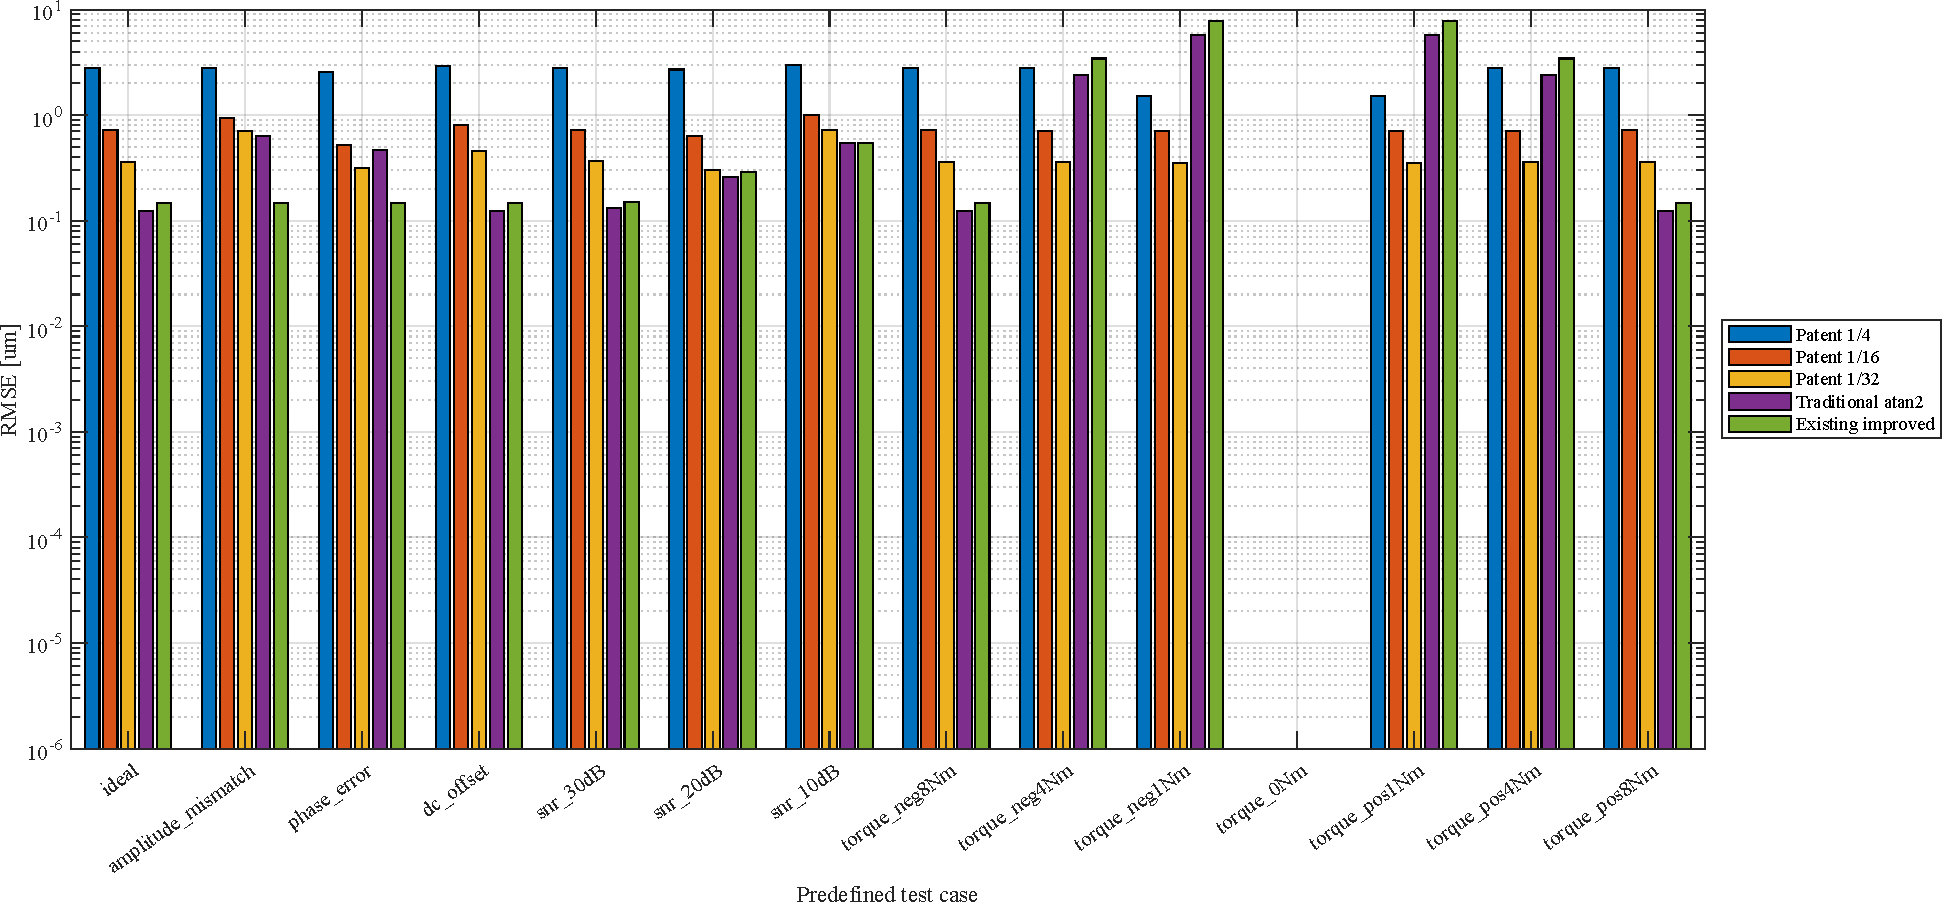
\includegraphics[width=0.88\linewidth]{figures/stage14_rmse_all_cases.pdf}
  \bicaption{14类典型工况下五种解调算法的位移RMSE横向对比}{Comparison of displacement RMSE among five demodulation algorithms across 14 operating conditions}
  \label{fig:rmse_all}
\end{figure}

\begin{table}[htbp]
  \centering
  \bitablecaption{五种解调算法在全工况下的统计性能与鲁棒性汇总}{Statistical performance and robustness summary of five demodulation algorithms under all conditions}
  \label{tab:method_summary}
  \resizebox{\textwidth}{!}{%
  \begin{tabular}{lcccccc}
    \toprule
    解调算法 & 有效工况 & 平均RMSE/$\mathrm{\mu m}$ & 中位数RMSE/$\mathrm{\mu m}$ & 最大RMSE/$\mathrm{\mu m}$ & 鲁棒性均值 & 最差工况 \\
    \midrule
    Patent 1/4 & 14/14 & $2.419$ & $2.808$ & $3.009$ & $0.256$ & snr\_10dB \\
    Patent 1/16 & 14/14 & $0.686$ & $0.712$ & $1.007$ & $0.500$ & snr\_10dB \\
    Patent 1/32 & 14/14 & $0.384$ & $0.360$ & $0.728$ & $0.638$ & snr\_10dB \\
    Traditional atan2 & 14/14 & $1.334$ & $0.365$ & $5.698$ & $0.578$ & torque\_neg1Nm \\
    Existing improved & 14/14 & $1.730$ & $0.148$ & $7.748$ & $0.565$ & torque\_neg1Nm \\
    \bottomrule
  \end{tabular}%
  }
\end{table}

由图\ref{fig:rmse_all}与表\ref{tab:method_summary}分析可知：
（1）Patent 1/32细分算法展现出优异的稳定性能，其全工况平均RMSE仅为$0.384\,\mathrm{\mu m}$，显著优于Patent 1/4（$2.419\,\mathrm{\mu m}$）和Patent 1/16（$0.686\,\mathrm{\mu m}$）。其步进量化机制天然具备高频噪声平滑能力，即使在信噪比恶化至$10\,\mathrm{dB}$的极端工况下，最大误差仍被严格抑制在$0.728\,\mathrm{\mu m}$以内；
（2）经典atan2算法与改进椭圆拟合算法在中低噪声工况下具有极高的局部辨识精度（中位数RMSE低至$0.148\,\mathrm{\mu m}$），但在强反向扭矩及非对称负载工况下出现较为明显的相位展开畸变，最大RMSE分别放大至$5.698\,\mathrm{\mu m}$与$7.748\,\mathrm{\mu m}$。

\subsection{动态跟踪误差曲线与演化机理分析}
五种算法在典型工况下的动态位移跟踪残差演化曲线如图\ref{fig:error_curves}所示。

\begin{figure}[htbp]
  \centering
  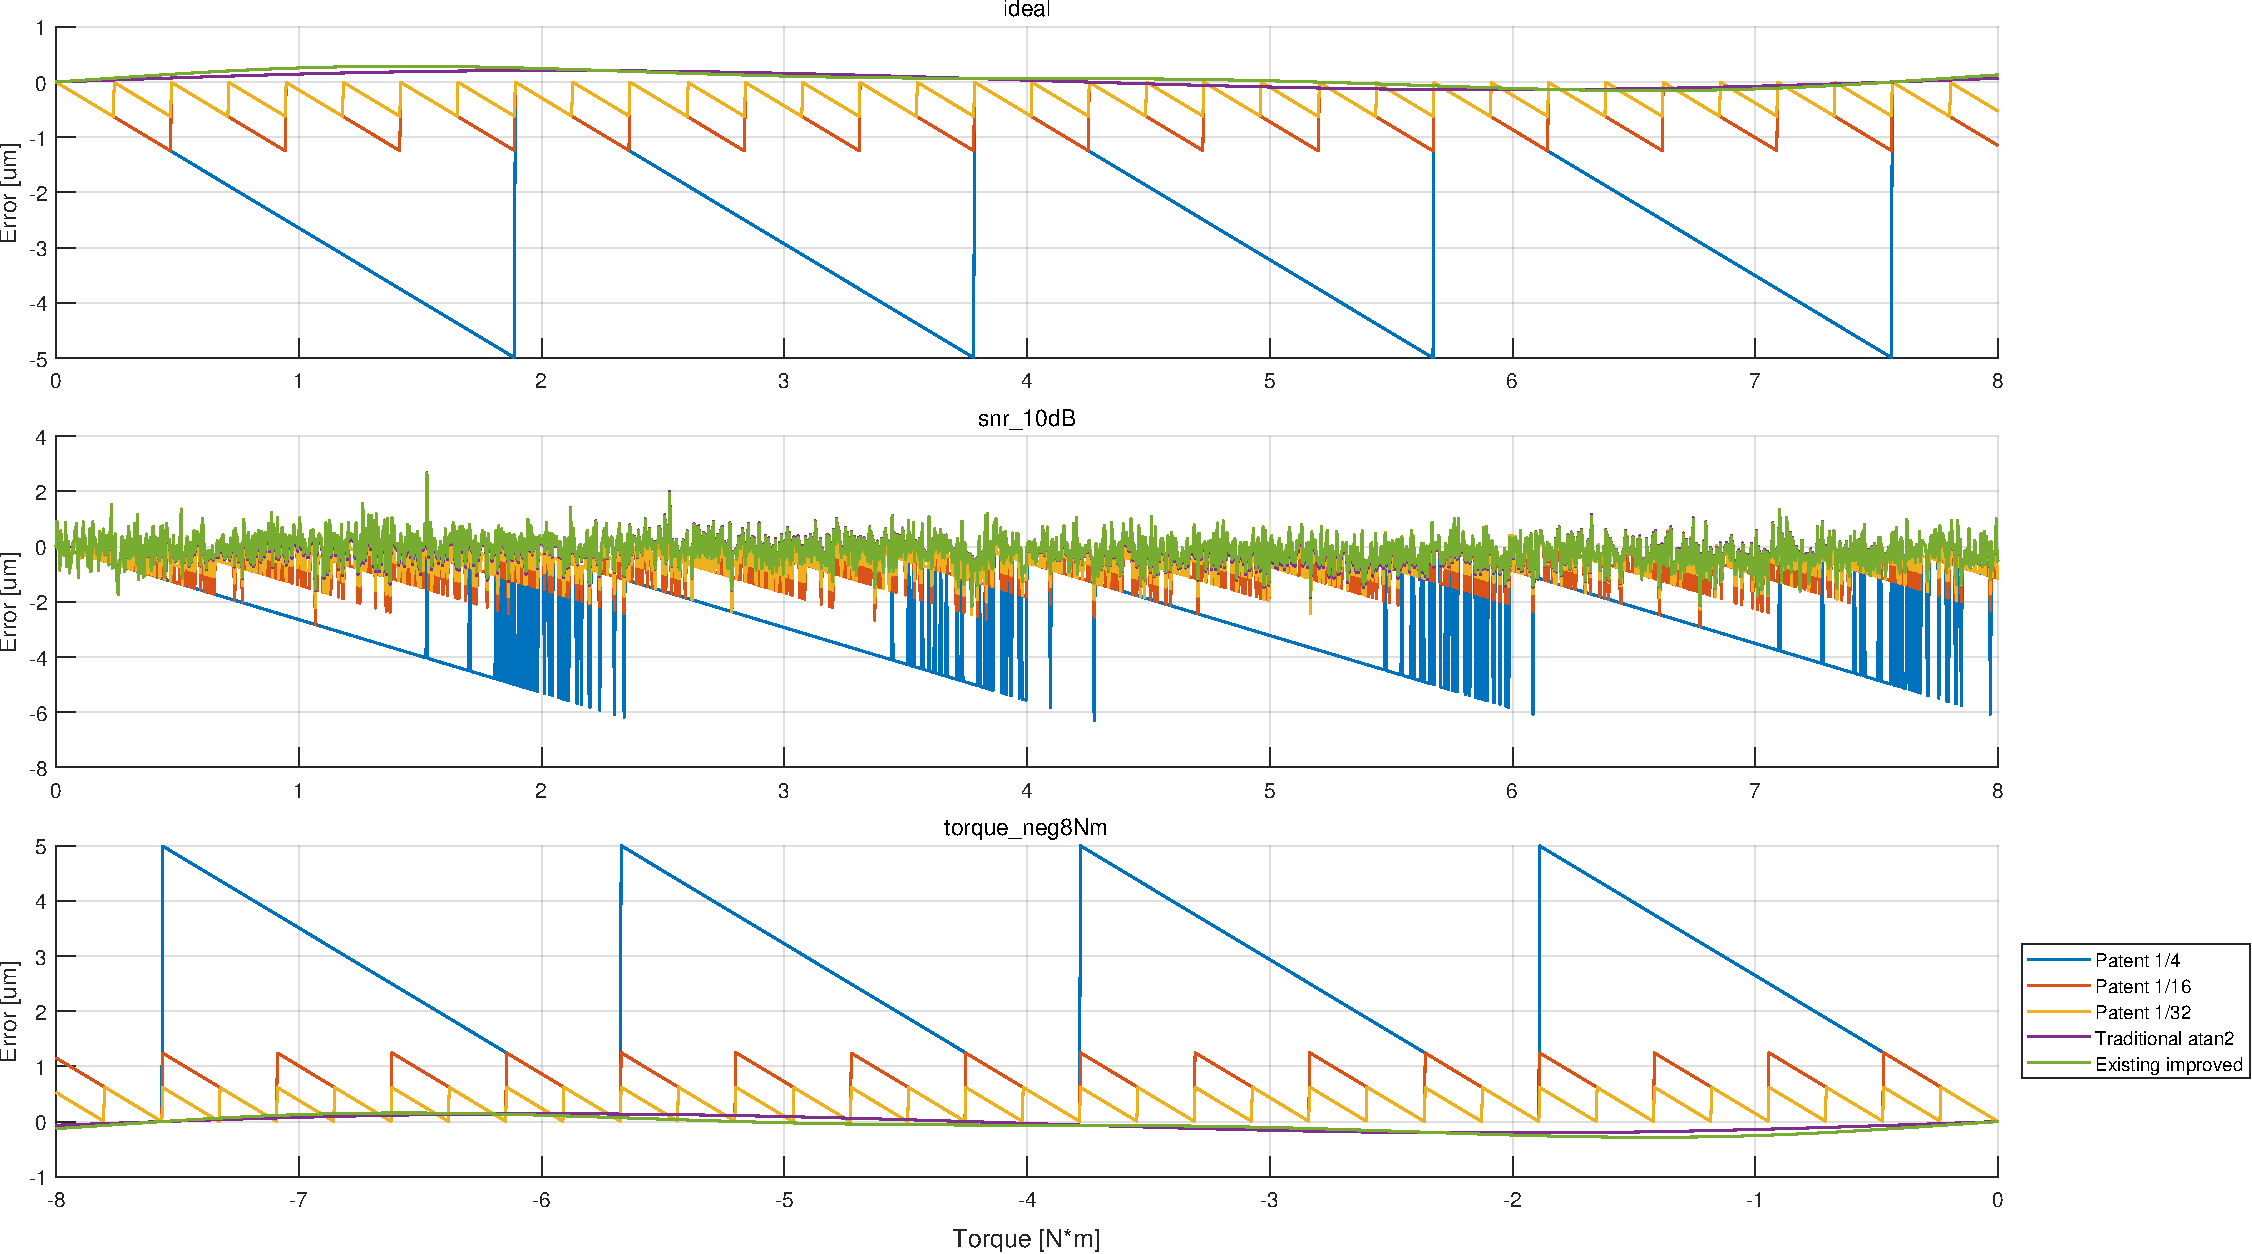
\includegraphics[width=0.88\linewidth]{figures/stage14_error_curves.pdf}
  \bicaption{典型工况下五种解调算法的瞬时位移估计残差曲线}{Instantaneous displacement estimation error curves of five demodulation algorithms under typical conditions}
  \label{fig:error_curves}
\end{figure}

如图\ref{fig:error_curves}所示，Patent 1/4至1/32系列计数输出呈阶梯状，残差反映了完成区间计数的量化特性；连续反正切类算法则表现为连续相位估计误差。对于当前脚本中的反向扭矩扫掠，这些曲线描述的是该采样窗口和unwrap实现下的结果，不外推为所有动态反向工况的普适结论。

\subsection{鲁棒性评分与抗噪鲁棒性评价}
为量化评价算法在扰动下的品质衰减，定义归一化鲁棒性评分为$S_{\mathrm{rob}} = 1 / [1 + \mathrm{RMSE} / (P / 32)]$。不同工况下各算法的鲁棒性得分分布如图\ref{fig:robustness}所示。

\begin{figure}[htbp]
  \centering
  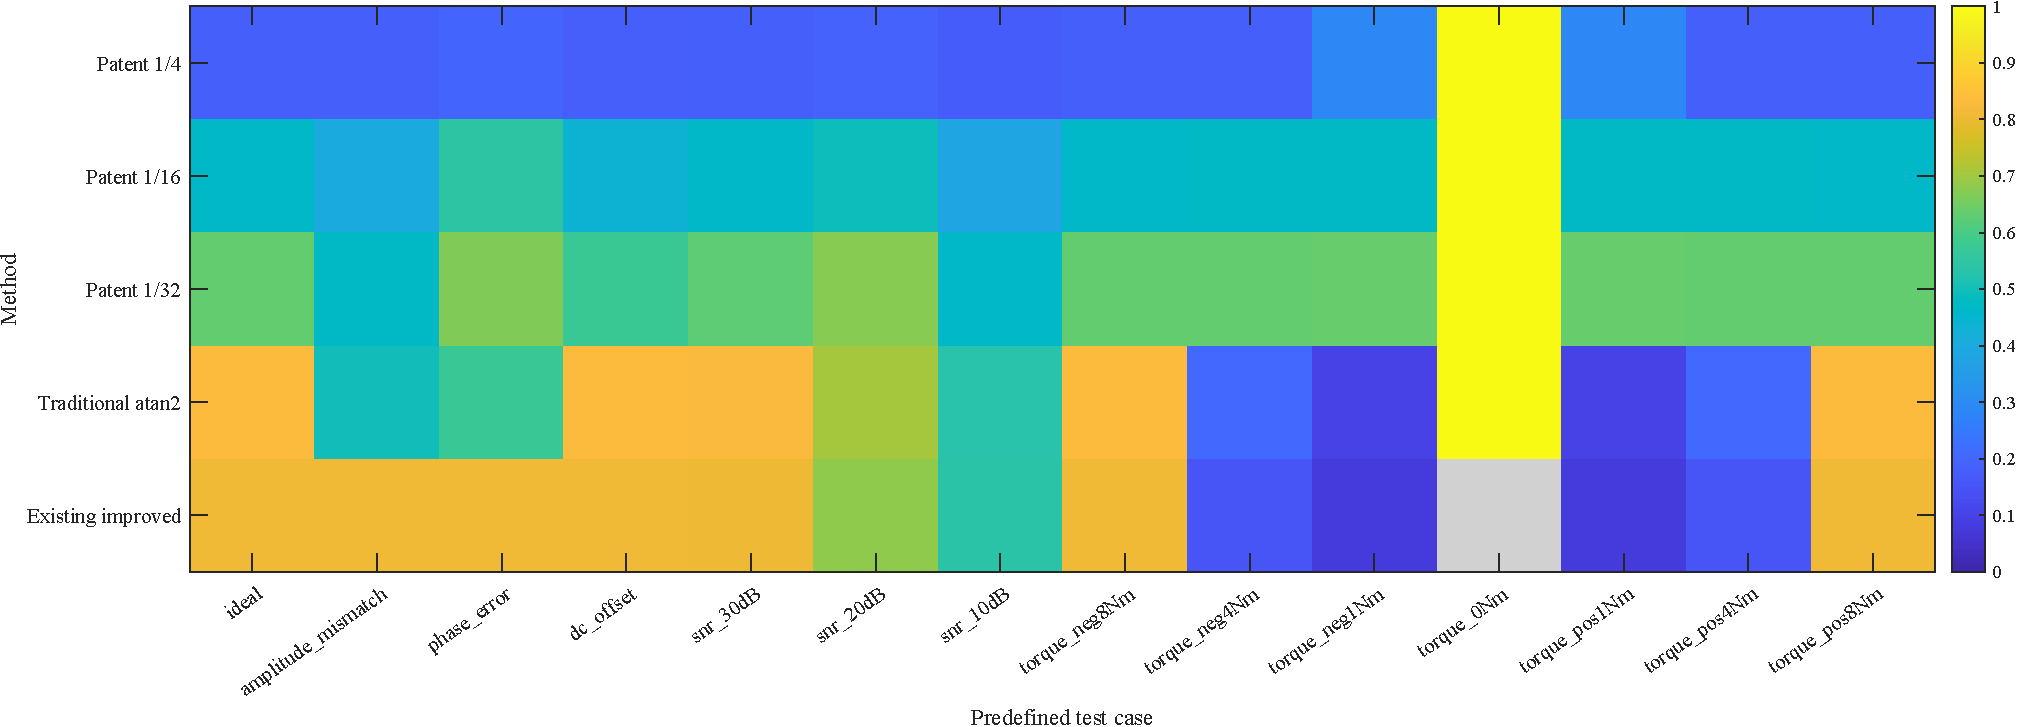
\includegraphics[width=0.85\linewidth]{figures/stage14_robustness_score.pdf}
  \bicaption{不同扰动工况下解调算法的综合鲁棒性评分分布}{Distribution of comprehensive robustness scores for demodulation algorithms under different conditions}
  \label{fig:robustness}
\end{figure}

如图\ref{fig:robustness}所示，Patent 1/32算法在当前14个离线工况中的归一化评分均值为0.638。该分数依赖预先选定的$P/32$归一化尺度，仅用于本组算法相对比较。

\subsection{零扭矩静态奇异点秩亏反常工况探讨}
在零扭矩恒定输入窗口测试中，现有白化算法可能触发底层线性代数的秩亏警告。某次运行记录为“MATLAB:rankDeficientMatrix: 秩亏，秩 = 1，tol = 1.987517e-11”；该数值依赖样本窗口和实现版本。

当输入在整个窗口恒为零且噪声为零时，四相信号不随时间变化，二维轨迹退化为单点；协方差矩阵因而失去足够的独立方向，白化步骤会变得病态。差分atan2和完成区间计数在该特定测试中仍能输出有限结果，但这只说明当前实现的数值行为，不能替代静态噪声和启动状态下的实机验证。

% ==================================================
% 4 环境温度特性与数字孪生在线补偿验证
% ==================================================
\section{环境温度特性与模型逆变换分析}

\subsection{宽温域下剪切模量与光栅周期漂移特性}
针对航天及车载极端工作温区，平台在$-20~^\circ\mathrm{C}\sim +80~^\circ\mathrm{C}$（步长$20~^\circ\mathrm{C}$）宽温域范围内开展了温度漂移机理仿真。材料剪切模量变化及综合灵敏度偏差率变化曲线如图\ref{fig:temp_sens}所示。

\begin{figure}[htbp]
  \centering
  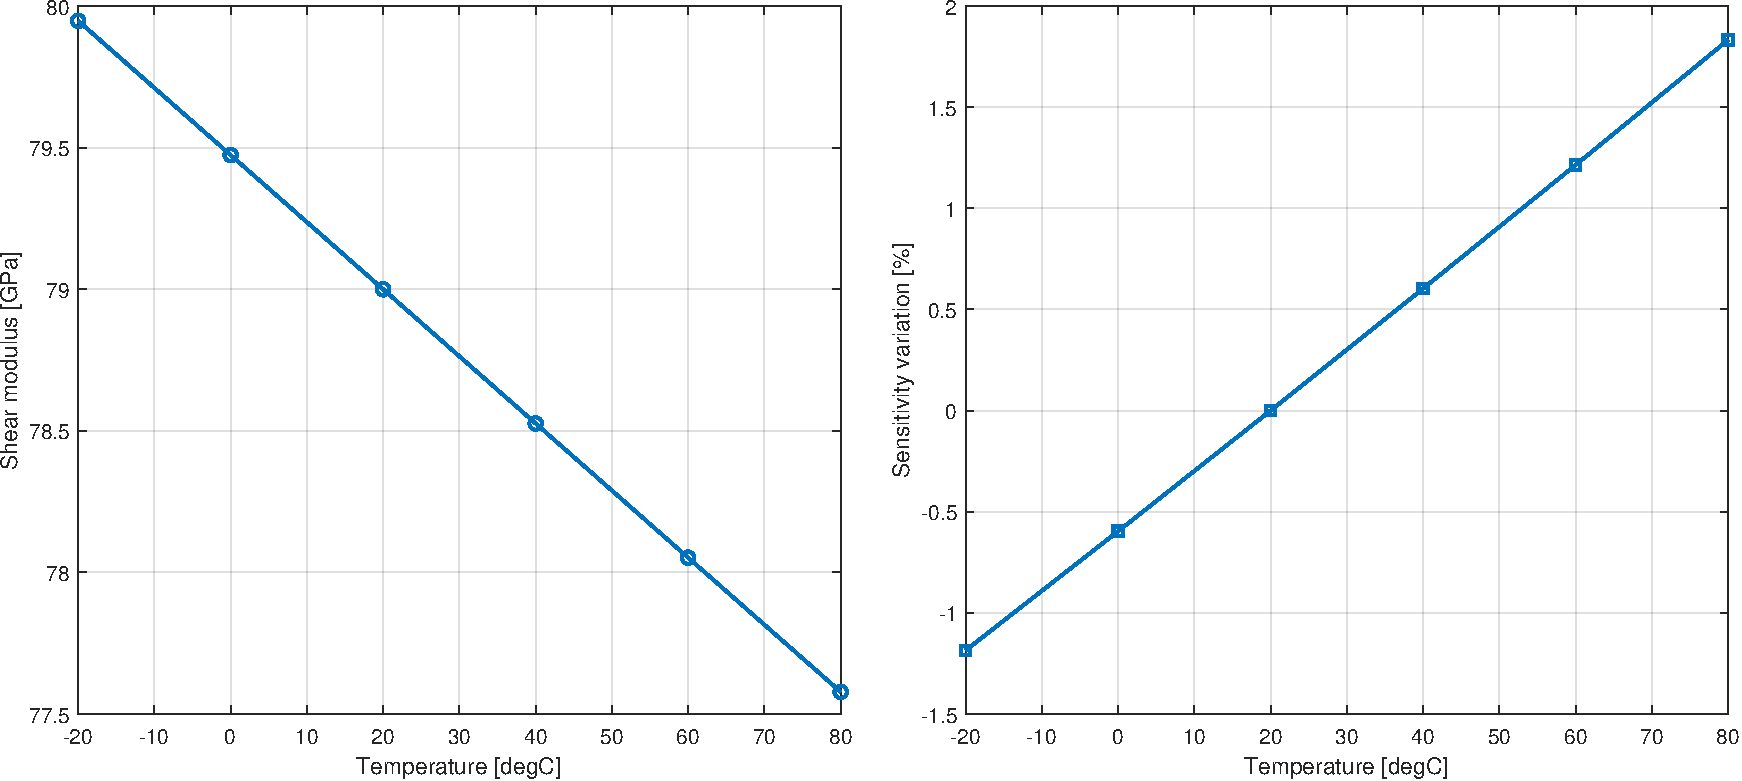
\includegraphics[width=0.82\linewidth]{figures/stage15_material_sensitivity.pdf}
  \bicaption{温度变化对材料剪切模量及测量灵敏度的影响曲线}{Effect of temperature variation on material shear modulus and measurement sensitivity}
  \label{fig:temp_sens}
\end{figure}

如图\ref{fig:temp_sens}所示，随着温度自基准温度$20~^\circ\mathrm{C}$升至$+80~^\circ\mathrm{C}$，扭轴剪切模量由$79.00\,\mathrm{GPa}$单调衰减至$77.58\,\mathrm{GPa}$，系统灵敏度发生$+1.83\%$的正向漂移；当温度降至$-20~^\circ\mathrm{C}$时，剪切模量硬化增大至$79.95\,\mathrm{GPa}$，灵敏度漂移达$-1.19\%$。

\subsection{温度参数逆变换前后精度对比}
采用式\eqref{eq:temp_comp}的同模型逆变换进行离线补偿。补偿开启（Compensation ON）与未补偿（Compensation OFF）状态下的扭矩RMSE对比曲线如图\ref{fig:comp_rmse}所示。全温区详细误差数值记录如表\ref{tab:temp_summary}所示。

\begin{figure}[htbp]
  \centering
  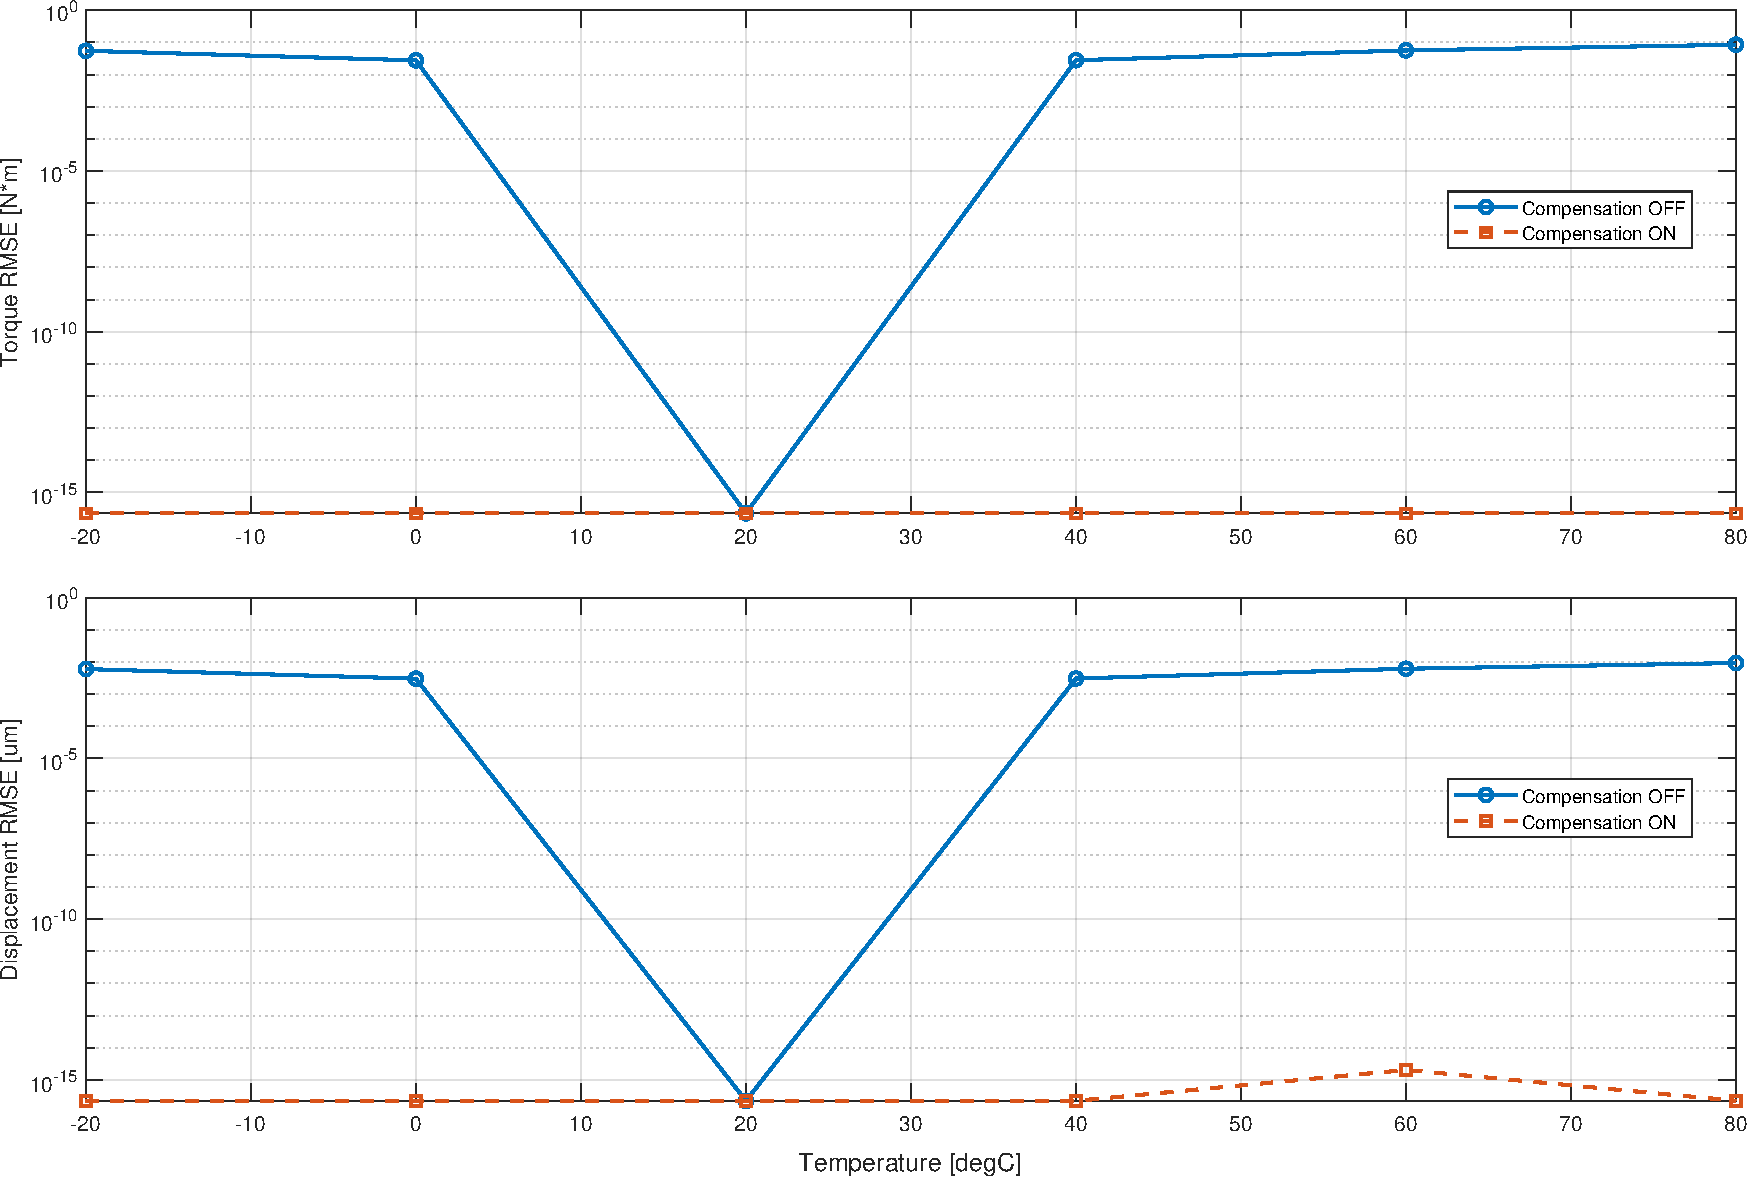
\includegraphics[width=0.82\linewidth]{figures/stage15_compensation_rmse.pdf}
\bicaption{温度模型逆变换前后扭矩RMSE对比}{Torque RMSE before and after inversion of the temperature model}
  \label{fig:comp_rmse}
\end{figure}

\begin{table}[htbp]
  \centering
  \bitablecaption{不同温度工况下系统温漂与数字孪生补偿效果对比}{Comparison of system thermal drift and digital twin compensation performance under different temperatures}
  \label{tab:temp_summary}
  \resizebox{\textwidth}{!}{%
  \begin{tabular}{cccccc}
    \toprule
    环境温度/$^\circ\mathrm{C}$ & 剪切模量/$\mathrm{GPa}$ & 灵敏度相对偏差/\% & 未补偿扭矩RMSE/$\mathrm{N\cdot m}$ & 补偿后扭矩RMSE/$\mathrm{N\cdot m}$ & 补偿后位移RMSE/$\mathrm{m}$ \\
    \midrule
    $-20$ & $79.95$ & $-1.186$ & $0.0548$ & $0.0000$ & $0.000$ \\
    $0$ & $79.47$ & $-0.596$ & $0.0275$ & $0.0000$ & $0.000$ \\
    $+20$ (基准) & $79.00$ & $0.000$ & $0.0000$ & $0.0000$ & $0.000$ \\
    $+40$ & $78.53$ & $+0.604$ & $0.0279$ & $0.0000$ & $0.000$ \\
    $+60$ & $78.05$ & $+1.215$ & $0.0561$ & $<10^{-20}$ & $<10^{-20}$ \\
    $+80$ & $77.58$ & $+1.833$ & $0.0847$ & $0.0000$ & $0.000$ \\
    \bottomrule
  \end{tabular}%
  }
\end{table}

由图\ref{fig:comp_rmse}与表\ref{tab:temp_summary}可知：
（1）在未实施补偿时，温漂引入的扭矩测量误差随温差扩大呈线性加剧，在$+80~^\circ\mathrm{C}$时扭矩测量RMSE高达$0.0847\,\mathrm{N\cdot m}$，最大瞬时误差达到$0.1408\,\mathrm{N\cdot m}$，严重超出了精密测量允许公差；
（2）采用同一参数模型进行逆变换后，表中补偿误差降至双精度浮点计算的舍入误差量级（部分点记录为$<10^{-20}\,\mathrm{N\cdot m}$）。这验证的是模型内部的可逆性；由于温度系数标注为未验证，不能据此声称实物温漂已被完全消除。

\subsection{仿真与物理验证边界}
本文使用的MATLAB模块能够生成ADC码和11字节四通道协议帧，也保留了图形界面和串口接口的扩展位置；本稿没有报告与物理样机、真实串口设备或FPGA的连接结果。因此，结构尺寸、$G$和$P$的温度系数均属于\texttt{simulation/default}假设，温度补偿和鲁棒性结果是离线模型验证，后续仍需用台架数据标定参数并进行独立硬件验证。

% ==================================================
% 5 结论
% ==================================================
\section{结论}

针对光栅扭矩测量中的非理想信号失真与温度参数漂移问题，本文建立了可追溯的离线全链路模型，评测了5类解调算法在14个预定义工况下的数值表现，并验证了温度参数逆变换的模型一致性。本文得出以下结论：

（1）构建了涵盖机械扭转力学、圆光栅相对切向位移、多通道光电转换、非理想误差注入、ADC量化及二进制定长串口帧接口的参数化模型；

（2）在脚本定义的14个工况（含幅值/相位/偏置扰动、30/20/10 dB高斯噪声和扭矩扫掠）中，Patent 1/32的平均位移RMSE为$0.384\,\mathrm{\mu m}$，最大值为$0.728\,\mathrm{\mu m}$，归一化评分均值为0.638；

（3）在零扭矩恒定窗口中，四相信号轨迹退化使协方差白化步骤出现秩亏风险；差分atan2和完成区间计数在该离线测试中仍输出有限结果，但静态切换可靠性仍需实物验证；

（4）在温度系数为仿真默认值的条件下，$-20~^\circ\mathrm{C}\sim +80~^\circ\mathrm{C}$范围内完整相位链的灵敏度变化为$-1.19\%\sim +1.83\%$，未补偿扭矩RMSE最大为$0.0847\,\mathrm{N\cdot m}$；同模型逆变换使残差降至数值舍入误差量级，但该结果不替代实物温漂标定。

后续工作将依托本数字孪生平台生成的标准化数据帧，开展基于FPGA的高速定点化细分固件移植，并在物理旋转扭矩台架上进一步开展实测标定与硬件在环验证。

% ==================================================
% 页脚/文末作者与基金信息
% ==================================================
\vspace{1.5em}
\noindent\textbf{收稿日期：}2026-03-10\par
\noindent\textbf{基金项目：}国家自然科学基金资助项目（62073210）；内蒙古自然科学基金资助项目（2021MS06015）；内蒙古科技计划重大专项（2022CG0041）。\par
\noindent\textbf{作者简介：}张三（1990—），男，内蒙古赤峰人，讲师，硕士，主要从事光电精密测量、数字孪生与智能传感技术研究。\par
\noindent\textbf{通信作者：}李四（1975—），男，教授，博士，主要从事智能仪器与光机电一体化测控系统研究，E-mail: lisi@chifenghu.edu.cn。\par

% ==================================================
% 参考文献（顺序编码制，方括号上标）
% ==================================================
\bibliographystyle{gbt7714-numerical}
\bibliography{references}

\end{document}

